\ifx\wholebook\relax\else
\input{../Common.tex}
\input{../macroes.tex}
\begin{document}
\fi

\chapter{\newcommand{\replace}[2]{Composing}{Combining} Methods}\label{ch:composons}

\begin{chapterfigure}
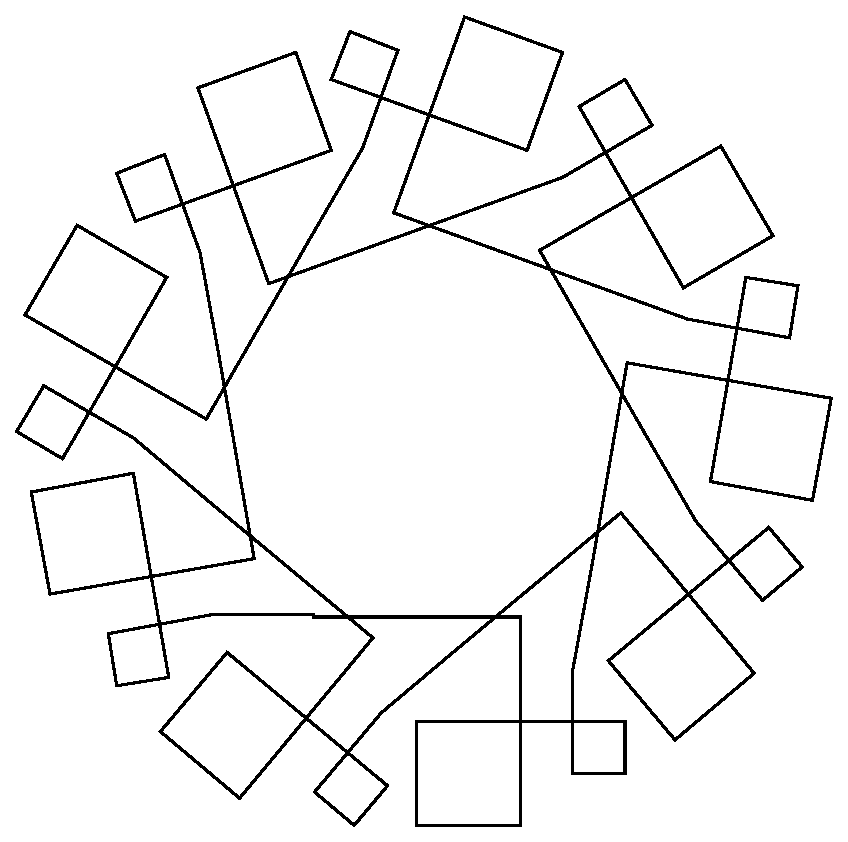
\includegraphics[width=6cm]{compArtNouveauTurningScr}
\end{chapterfigure}

In  Chapter~\ref{ch:turtleTeaching}, you learned how to define methods. We showed that defining methods is interesting because (1) methods avoid \newcommand{\replace}[2]{to have to rewrite}{rewriting} scripts and \newcommand{\replace}[2]{introduce}{introducing} errors and (2) methods can be used by different robots. The other main advantage of using methods \newcommand{\remove}[1]{that we are going to explore in this chapter} is the possibility \newcommand{\replace}[2]{to reuse}{of reusing} methods, \ie \newcommand{\replace}[2]{to define}{defining} a method by calling other methods. \newcommand{\add}[1]{Reuse is what we will explore in this chapter.\paragraph
}
Being able to reuse methods is extremely important because we can define a method in terms of another one\newcommand{\add}[1]{,} without having to know all the details of how the second method is defined.  We just call it.

\section{Nothing Really New: the \ct{square} Method}
Composing \newcommand{\replace}[2]{method}{methods} is quite natural and \newcommand{\remove}[1]{it} is not really new. \newcommand{\replace}[2]{Indeed, this}{Actually it} is what we \newcommand{\replace}[2]{made}{did} in Chapter~\ref{ch:turtleTeaching} when we defined a method! The method \ct{square} is defined by calling the methods \turnLeft and \timesRepeat. @@dank: omitting 'go:' from the list might confuse students by raising the question why it was left out -- I recommend including it.@@  \newcommand{\replace}[2]{Therefore it}{Even \ct{square}} is defined in terms of other
methods\newcommand{\replace}[2]{ but}{, and} we \newcommand{\replace}[2]{do not}{don't} have to know how \turnLeft or \timesRepeat are defined. So we are already done with this chapter!

\begin{method}\label{comp:square}
square 
   "Draw a square of 100 pixel size"

   4 timesRepeat: 
         [ self go: 100;
                  turnLeft: 90]
\end{method}


\section{Other Graphical Patterns}
In Chapter~\ref{ch:turtleTeaching}, we \newcommand{\replace}[2]{asked you to define}{defined} the method \ct{pattern} that draws a nice pattern (See~\scrref{src:artNouveau}). Now we ask you to \newcommand{\replace}[2]{follow the experiments}{experiment} and produce the \newcommand{\add}[1]{following} drawings by defining \newcommand{\replace}[2]{following}{more} methods. 

%We remind you the definition of this method if you forgot to save it, so that you can define it now. 
%\begin{methodfig}{compArtNouveauScr}\label{src:mth:artnouveau}
%artNouveau
%   "draws a thing"

%   self go: 100.
%   self turnRight: 90.
%   self go: 100.
%   self turnRight: 90.
%   self go: 50.
%   self turnRight: 90.
%   self go: 50.
%   self turnRight: 90.
%   self go: 100.
%   self turnRight: 90.
%   self go: 25.
%   self turnRight: 90.
%   self go: 25.
%   self turnRight: 90.
%   self go: 50
%\end{methodfig}



\begin{exofigwithsize}[0.5]{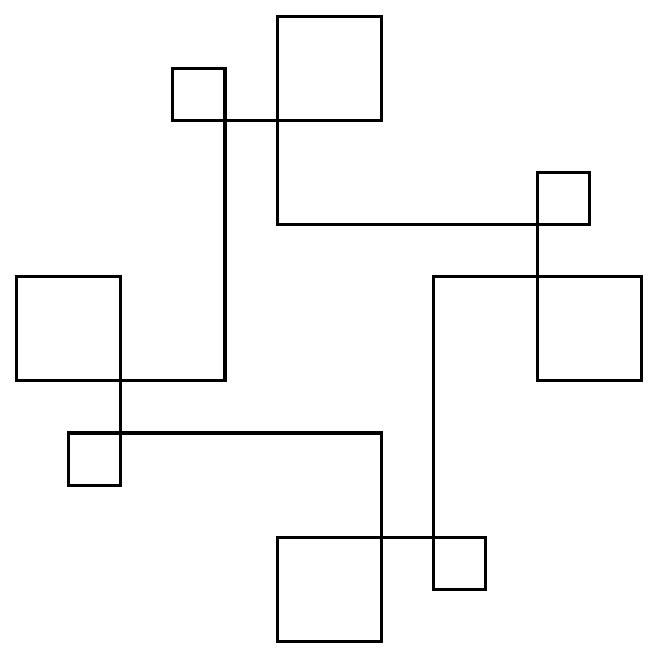
\includegraphics[width=5cm]{compCompleteThing}}
Define the method \ct{pattern4} that calls \newcommand{\replace}[2]{4 times \ct{pattern} and produces right figure and that we use  in the script below}{\ct{pattern} 4 times to produce the figure on the right. \paragraph
We will also use this method in another script later.} 

\begin{nalltt}
| \caro |
\caro := \Turtle new.
\caro pattern4
\end{nalltt}
\end{exofigwithsize}

\begin{exonofig}
Define the method \ct{tiltedPattern}  draws the \newcommand{\replace}[2]{first picture of the}{picture at the beginning of this} Chapter. \newcommand{\replace}[2]{To help you a bit you have a repeat 9 times the pattern}{Hint: you have to repeat the pattern 9 times,} and the angle to turn is 10 degrees.

\end{exonofig}

\hidden{\begin{nalltt}
tiltedPattern 

   9 timesRepeat: 
                  [self pattern. 
                  self turnRight: 10. 
                  self go: 50 ]
\end{nalltt}}


\begin{exofigwithsize}[0.5]{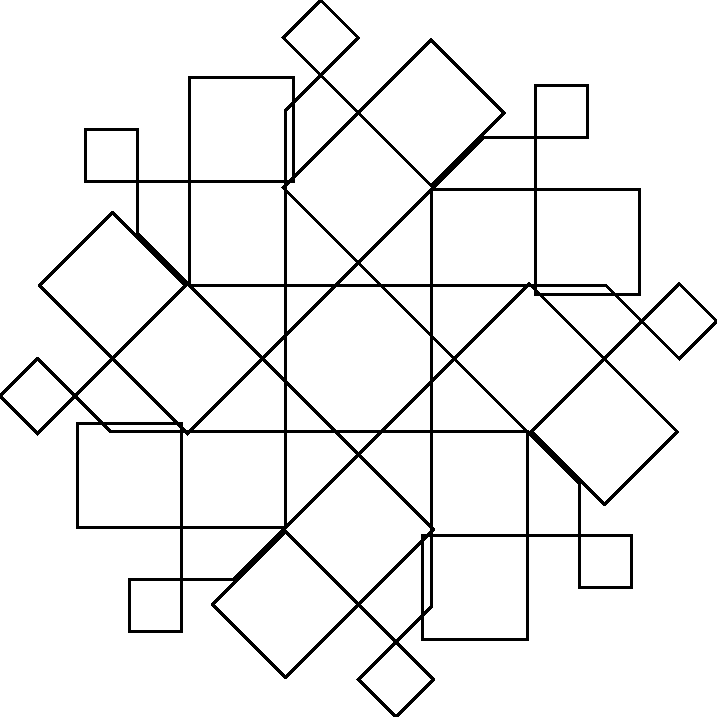
\includegraphics[width=6cm]{compArtNouveauGiantScr}}
Define the method \ct{doubleFrame} that draws the picture on the right. 

\

\begin{nalltt}
doubleFrame

    8 timesRepeat: [self pattern ;
                                     turnLeft: 45 ;
                                     go: 100]
\end{nalltt}
\end{exofigwithsize}


\section{Stepping Back}
Now \newcommand{\replace}[2]{let us analyze what we learned}{let's see what we can learn} from the experiments you did. As you can see \newcommand{\replace}[2]{it with}{from} the methods \ct{pattern4}, \ct{tiltedPattern}, and \ct{doubleFrame}, the method \ct{pattern} is only defined once, \newcommand{\replace}[2]{but}{and then} reused several times in different methods. Defining \ct{pattern} as a method allows you to: (1) define it only
once, (2) reuse it in various contexts and (3) \newcommand{\remove}[1]{do} not introduce errors during the rewriting of this method. 

If you look at the definition of the method \ct{doubleFrame}, you see that it is defined in terms of \newcommand{\add}[1]{the} \ct{pattern} method that is itself defined in terms of other methods such as \go, \turnLeft...\newcommand{\add}[1]{ }and so on. In fact, a complex method is often defined in terms of simpler methods, which \newcommand{\replace}[2]{as well}{themselves} are defined in terms of \newcommand{\add}[1]{even} simpler methods \newcommand{\replace}[2]{too}{---} and so on. This is because it is \newcommand{\replace}[2]{simpler}{easier} to understand and to define simpler methods.  In Chapter~\ref{ch:recomposing} we shall show you that to solve a problem it is simpler to decompose it \newcommand{\replace}[2]{in terms of}{into} smaller subproblems, solve them and \newcommand{\add}[1]{then} use them to finally solve the first problem. 

It is essential to understand that while defining the method \ct{doubleFrame} we do not \newcommand{\add}[1]{have} to know how \ct{pattern} is defined, we just \newcommand{\replace}[2]{want}{need} to know what \newcommand{\replace}[2]{is}{it} does and \newcommand{\add}[1]{how} to use it!  When we define a method we are giving a name to a sequence of messages \newcommand{\replace}[2]{and doing so we are reducing}{, which reduces} the number of details that we have to remember.  We just have to remember what \newcommand{\remove}[1]{does} the method \newcommand{\add}[1]{does} and its name\newcommand{\add}[1]{,} not how it does it.  We say that we are building an \emph{abstraction} over the definition details.

To \newcommand{\replace}[2]{really show you}{make} this point\newcommand{\add}[1]{ clear}, we rewrote the method
\ct{doubleFrame} without calling the method \ct{pattern}\newcommand{\replace}[2]{, we directly copied}{ by directly copying} the definition of \newcommand{\replace}[2]{this method}{\ct{pattern}} (shown in italic) inside the other one. Compare \newcommand{\add}[1]{\ct{doubleFrameWithoutCallingPattern}} with the method \ct{doubleFrame}\newcommand{\replace}[2]{ and}{. The new version without \ct{pattern} is not only longer --- for most people it is also more confusing and harder to understand. \paragraph

Now} imagine \newcommand{\replace}[2]{that we would do}{what would happen if we did} the same with the code of \turnRight, \turnLeft, and \go \newcommand{\add}[1]{---} because \newcommand{\replace}[2]{there}{these} are \newcommand{\remove}[1]{also} methods\newcommand{\add}[1]{ too}. \newcommand{\replace}[2]{This}{It} would be a nightmare\newcommand{\replace}[2]{.}{!} There would be so \newcommand{\replace}[2]{much}{many} details that we would be lost all the time. 

\begin{method}
\newcommand{\replace}[2]{doubleFrameWithoutCallingArtNouveau}{doubleFrameWithoutCallingPattern}

   8 timesRepeat: [\textit{self go: 100.
                  self turnRight: 90.
                  self go: 100.
                  self turnRight: 90.
                  self go: 50.
                  self turnRight: 90.
                  self go: 50.
                  self turnRight: 90.
                  self go: 100.
                  self turnRight: 90.
                  self go: 25.
                  self turnRight: 90.
                  self go: 25.
                  self turnRight: 90.
                  self go: 50thing.}
                  self turnLeft: 45. 
                  self go: 100]
\end{method}



\largecadre{We define a method in terms of other ones \newcommand{\remove}[1]{and this at various levels}
without having to know how \newcommand{\replace}[2]{these}{the other} methods \newcommand{\remove}[1]{themselves} are defined. \newcommand{\add}[1]{We can do this repeatedly and at more than one level.}}
@@dank: What about breaking this into three simpler statements?
When we write a new method, it can call other methods.
We can use a method without knowing how it is written.
After we finish writing a method, we can call it when we write another method.@@ 

\section{Squares Everywhere}
Now \newcommand{\replace}[2]{it is time for you to practice}{you can try it}. Define the following methods using the method \ct{square}.


@@dank: I recommend modifying the macro 'exonofig' to make the associated label (in this case 'Some Boxes.') visually distinct from the subsequent text; otherwise it blends in too much and looks like a sentence fragment.  Appending the label to the 'Experiment n.m' heading with a separating colon (like 'Experiment 14.4: Some Boxes') and all in the same font style, seems a good option.  Otherwise boldface text or a terminating line break would help.  The terminating period character '.' should probably be removed, but that might depend on the new format.@@  \begin{exonofig}{Some Boxes.}
Define the methods \ct{box} and \ct{separatedBox} that produce the 
pictures shown in Figure~\ref{c7groscarre}.
\end{exonofig}

\begin{figure}[!htbp]
\begin{minipage}[c]{.4\linewidth}
\centerline{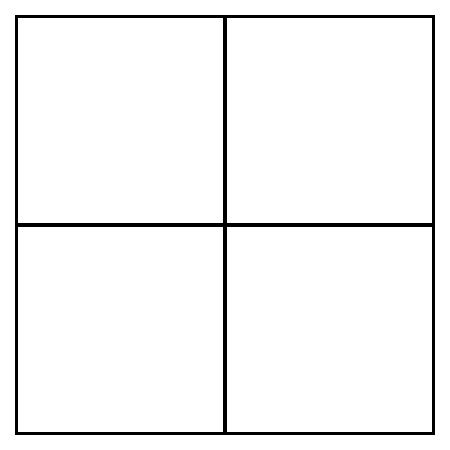
\includegraphics[width=\linewidth]{comp4Squares}}
\end{minipage}
\hfill
\begin{minipage}[c]{.4\linewidth}
\centerline{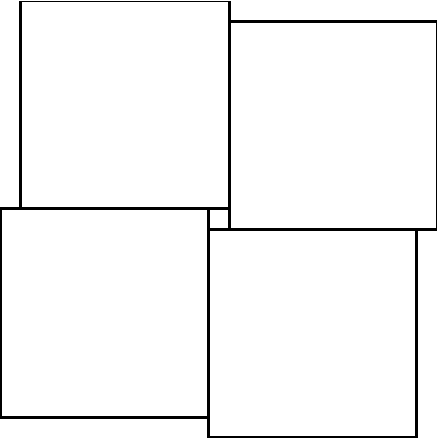
\includegraphics[width=\linewidth]{comp4SquaresTwo}}
\end{minipage}
\label{c7groscarre}
\end{figure}
 

\hidden{
| caro |
caro := Turtle new.
4 timesRepeat: [caro square100.
               caro turnLeft: 90]

| caro |
	caro := Turtle new.
	4 timesRepeat: 
		[ caro compSquareL100.
        caro turnLeft: 90. 
		caro go: 10]
}

\begin{exonofig}
\newcommand{\replace}[2]{Modifying}{Using} your previous methods to generate various figures.
\end{exonofig}

\hidden{
\begin{alltt}
| caro |
caro := Turtle new.
12 timesRepeat: [caro square100.
                caro turnLeft: 30.
                caro go: 10]
\end{alltt}}


\begin{exonofig}{Star.} 
Using the method \ct{box}, experiment and define a method \ct{star} that \newcommand{\replace}[2]{produce}{produces} the \newcommand{\replace}[2]{right}{right-hand} picture in Figure~\ref{c7star}\newcommand{\add}[1]{.}
\end{exonofig}

\begin{figure}[!htbp]
\begin{minipage}[c]{.4\linewidth}
\centerline{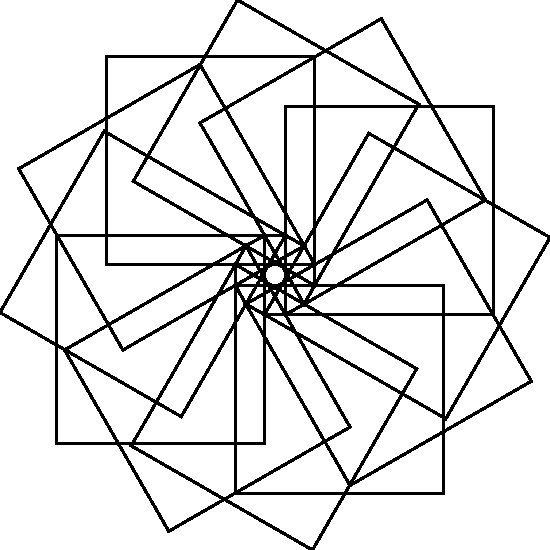
\includegraphics[width=5cm]{comp4SquaresThree}}
\end{minipage}
\hfill
\begin{minipage}[c]{.4\linewidth}
\centerline{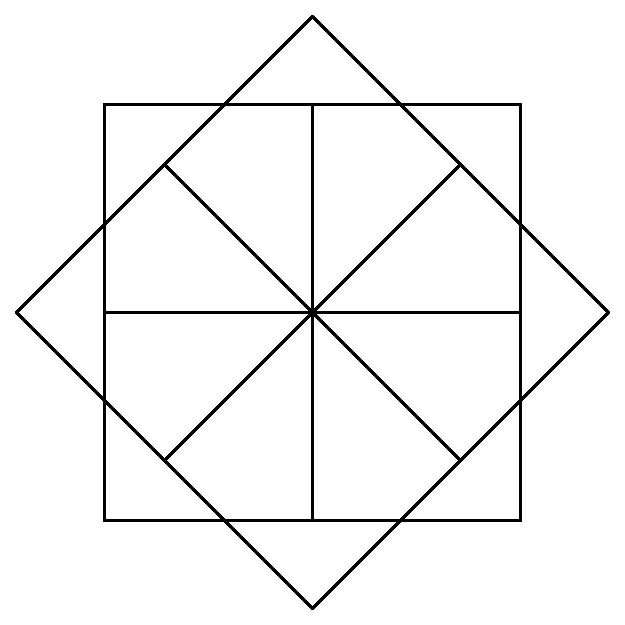
\includegraphics[width=5cm]{comp4SquaresFour}}
\end{minipage}
\label{c7star}
\caption{Stars}
\end{figure}


\summa

We can define a method in terms of other ones \newcommand{\remove}[1]{and this at various levels} without having to know how \newcommand{\replace}[2]{these}{the other} methods \newcommand{\remove}[1]{themselves} are defined.
\newcommand{\add}[1]{We can do this repeatedly and at more than one level.}

\ifx\wholebook\relax\else
\end{document}\fi
